\chapter{Estado del arte}\label{EdA}
%Función que crea el título de capítulo y al cual se le da el nombre deseado a través de su parámetro obligatorio. Al no tener la función el “*” se escribirá también en el título del documento las palabras “Capítulo 1: …”. Además se indica, mediante la función “\label”, la correspondiente etiqueta que lleva asociada. La etiqueta sirve para que en caso de que luego se quiera hacer referencia al capítulo se haga llamando etiqueta tal que se escribiría “La información correspondiente a dicho tema se encuentra en el capítulo \ref{Int}.”

\thispagestyle{fancy}
%Función que determina que durante este capítulo se aplique el estilo Fancy.

\fancyhead[LE]{\thechapter.Estado del arte} 

\section*{SSI}
SSI (Self sovereign identity) en ingles, es un un concepto en el la propia persona por existir, se representa a si mismo en internet. Esto, quiere decir que en internet nos dejaríamos de identificar utilizando correos electrónicos y pasaríamos a identificarnos por nuestra propia voluntad y una unión de clave publica y clave privada.

\section*{Introducción a las blockchain}
La blockchain, es un elemento importante para este proyecto. Su implementación, permite una comunicación segura y anónima entre personas, sin necesidad de ser verificada por terceros. Las blockchain, vienen en muchas formas y tipos, algunas siendo descentralizadas. Las mas populares, funcionan de manera puramente descentralizada, usando un sistema de prueba de trabajo para verificar todas las transacciones.
\subsection*{¿Que significa la descentralización en la red?}
Ser descentralizado, significa, que ninguna de las “personas” que participan en la red, tienen el control de la red. Es un proceso en el que el poder se reparte entre todas las personas de la red. Tradicionalmente, en el mundo financiero actual, esta controlado por los bancos. Actualmente, las personas de a pie no tenemos el poder de ser independientes a la hora de realizar pagos monetarios, ya que desde las monedas físicas hasta los pagos virtuales, están gestionados por ellos. Todo el poder monetario esta oculto en un grupo muy selecto de personas. Negando la posibilidad de decidir sobre nuestro dinero a ninguna de las personas de a pie.
Así mismo, desde un punto de vista de sistemas, un sistema P2P \ref{fg:decentralization_diagram} (peer to peer), permite hacer un sistema a prueba de fallos ya que en vez de necesitar un gran punto de enlace con el cual todas las personas se pueden conectar.
\begin{figure}[h!]
    \centering
    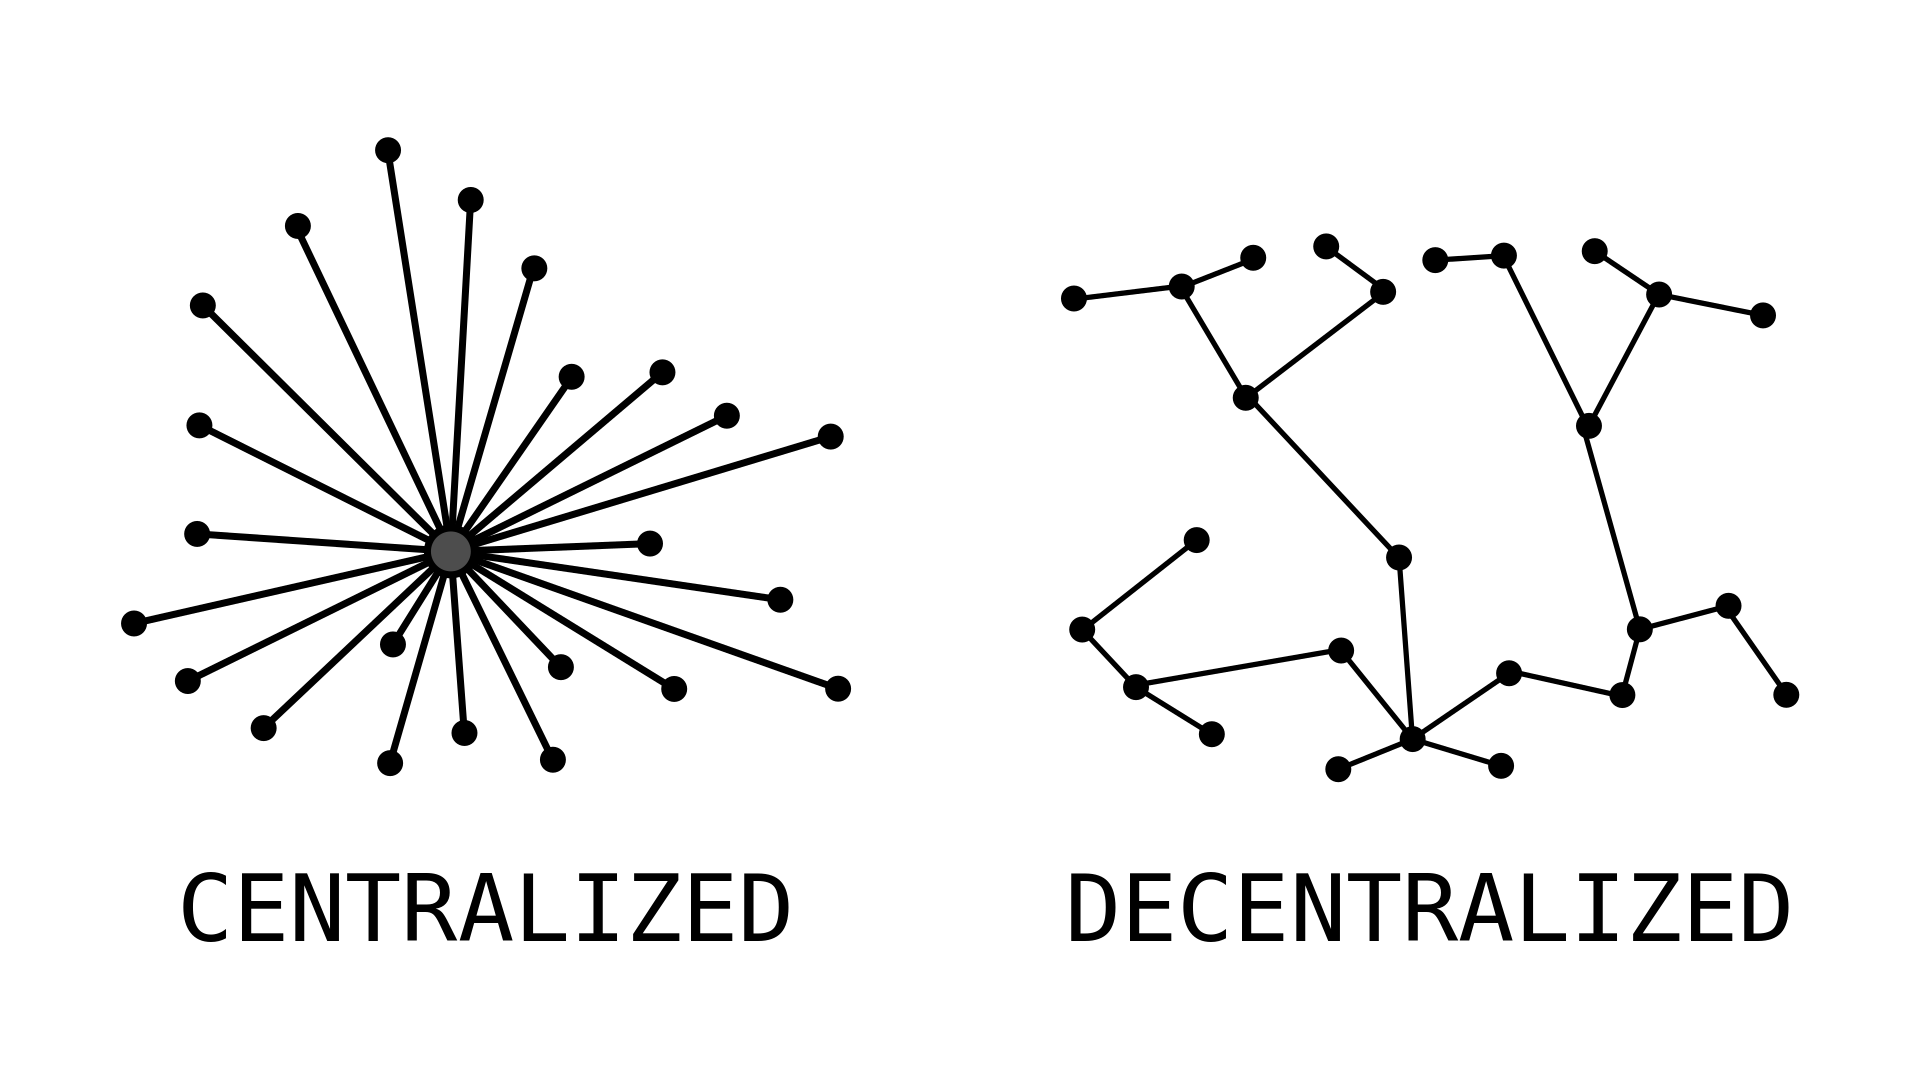
\includegraphics[width=0.7\textwidth]{Figures/Decentralization_diagram.png}
    \caption{Digrama explicando la descentralización}
    \label{fg:decentralization_diagram}
\end{figure}
Las criptomonedas, permiten liberarnos de los intermediarios. Consiguen que las transacciones se realicen entre dos personas sin necesidad de transmitir esa información por multiples canales para conseguir realizarla.
\subsection*{Ethereum}
Ethereum, es la evolución natural de Bitcoin. En su propio whitepaper, hablan de como bitcoin es un estado de transición. Justificando que ethereum, tiene mas bloques de construcción para permitir crear un internet descentralizado. Ethereum aporta cambios sustanciales a la forma en la que es minado y crea un nuevo concepto llamado smart contracts, que permiten la ejecución de código automática en respuesta a eventos que ocurren en la red.
Todos los eventos, son tratados como mensajes. Es un termino parecido a las “transacciones” clásicas en bitcoin. Estos mensajes, no son simplemente envíos de dinero, ya que pueden ser verdaderos mensajes enviados por smart contracts los cuales pueden responder. Haciendo a niveles prácticos una función a la que podemos llamar.
Una transacción, en ethereum tiene las siguientes partes:
\begin{center}
    \begin{tabular}{p{0.3\linewidth} | p{0.6\linewidth}}
        \hline
        Mensaje & Mensaje que quiere ser enviado \\
        \hline
        Firma   & Prueba criptográfica que verifica que el sender es quien dice ser. \\
        \hline
        Atributos especiales \\
        \hline
        STARTGAS &  Para evitar la ejecución de un bucle infinito en el minero, se impone un limite de gas que se va quemando mientras la ejecución avanza. Cuanto mas se tarde en ejecutar mas gas se quema. \\
        \hline
        GASPRICE & Por cada unidad de gas que es quemada, se le pagará al minero con su equivalencia en ether. \\
        \hline
    \end{tabular}
\end{center}
Gracias a estos atributos especiales, podemos generar una experiencia de usuario mejor.
\begin{itemize}
    \item Si alguna transacción llegase a fallar, se le devolvería el gas restante. Estos fallos, se pueden tirar con \texttt{require}. Esta keyword reservada espera un booleano con evaluación positiva.
Este código muestra \texttt{require} es funcionamiento.
\begin{lstlisting}
    function foo()
    public
    {
    // ... 
    // La ejecucion continua
    require(true,
    'Mensaje para enviar al sender si llega a fallar');
    // Si algun check llega a fallar se revierte el estado 
    require(false,
    'El sender vera este mensaje ya que el booleano es falso');
    // ...
    }
\end{lstlisting}
    \item Si alguna transacción se queda sin gas, el estado se revierte al inicial pero el dinero es perdido.
\end{itemize}

\subsection*{Minería}
La minería es el concepto de verificar las transacciones que ocurren en la red. A día de publicación de este trabajo, el sistema de verificación que utiliza es proof-of-work. Al utilizar el mismo mecanismo de protección, sus transacciones se parecen.
\begin{figure}[h!]
    \centering
    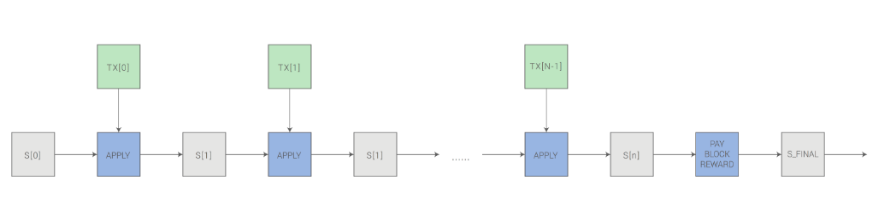
\includegraphics[width=0.8\textwidth]{Figures/Screenshot_20220507_131504.png}
    \caption{Diagrama que explica la mineria}
    \label{fg:block_diagram}
\end{figure}
La red de ethereum, siempre se asegura que se genera un bloque cada 12 segundos.
Estos 12 segundos son una especie de latido que muestra la salud de la red de ethereum. Para mantener siempre ese ritmo, se ajusta la dificultad de minado.
\begin{enumerate}
    \item Se genera una transacción y se firma con la clave privada.
    \item El usuario comparte la petición a toda la red de ethereum desde un minero.
    \item En algún momento de esos 12 segundos, un minero puede llegar a agregar cientos de transacciones en un posible bloque, en una manera que maximiza las comisiones de transacción. Todo esto mientras están por debajo del limite de gas.
    \begin{enumerate}
        \item Verifica la legitimidad de la transacción. i.e la firma corresponde al mensaje y si la cuenta tiene liquidez.
        \item Inicia el proceso de proof of work. Este proceso se basa en los siguientes parámetros. Dificultad del bloque ex. \texttt{3,324,092,183,262,715}, mixHash ex.\\ \texttt{0x44bca881b07a6a09f83b130798072441705d9a665c5ac8bdf2f39a3cdf3bee29} y la sal (numero hexadecimal aleatorio) \texttt{0xd3ee432b4fb3d26b}. Proof of work es una carrera entre todos los mineros de la red para ver quien puede generar. Cuando se genera un hash con SHA 256 ex. \\\texttt{ba7816bf8f01cfea414140de5dae2223b00361a396177a9cb410ff61f20015ad} se busca que un hash con una cierta cantidad de ceros al principio. La dificultad del bloque es cuantos hashes se pueden ser correctos para ese bloque. Cuanto menor sea el numero mas difícil es verificar ese bloque.
    \end{enumerate}
    \item Eventualmente, algún minero conseguirá solucionar el puzzle criptográfico y nuestro mensaje estará aceptado en la blockchain. Ese bloque contiene el checksum de todas los elementos internos.
    \item El resto de la red, al escuchar que un minero ha conseguido solucionar el bloque, lo verifica y si es correcto lo toma como el estado canónico de la red.
    \item Por ultimo los mineros borran de su memoria la lista de su mempool.
\end{enumerate}
\subsection*{Gas}
Como se ha explicado antes, se puede ejecutar código en la red de ethereum. Para proteger la red, existe una pequeña tarifa que hay que pagar por cada momento de ejecución. Así se evitan la existencia de ataques por parte de actores malignos.
Cuando una transacción se completa, se envía de vuelta el gas resultante al origen \ref{fg:message_diagram}.
\begin{figure}[h!]
    \centering
    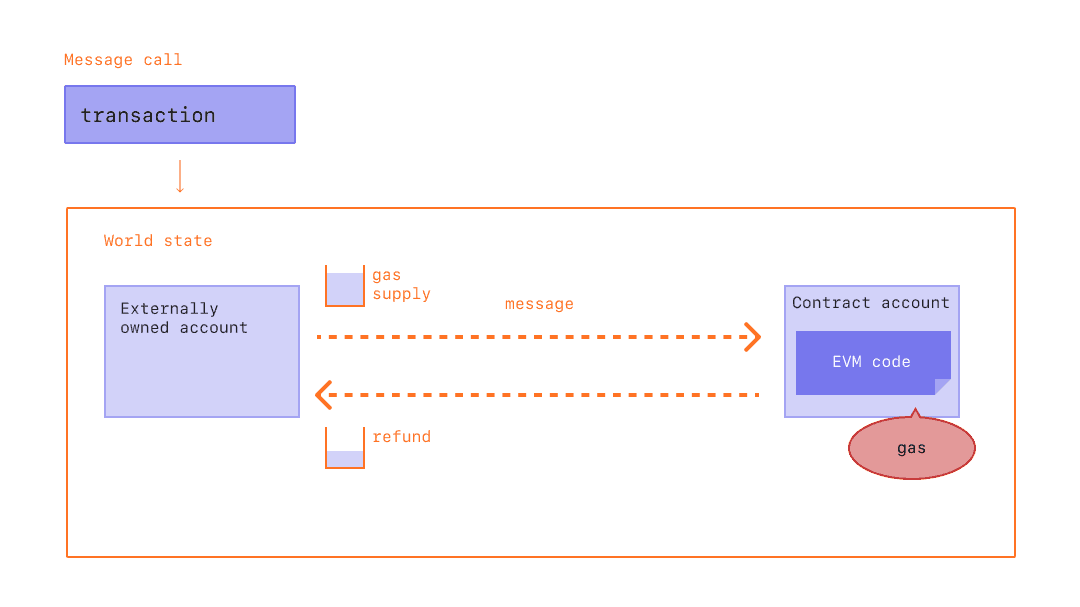
\includegraphics[width=0.8\textwidth]{Figures/gas-tx.png}
    \caption{Diagrama que explica el uso de gas}
    \label{fg:message_diagram}
\end{figure}
\begin{equation}
    max fee - (base fee + tip) = refund
\end{equation}
Después de la “London update”, el gas en ethereum ha evolucionado para proteger mas a los usuarios de posibles manipulaciones por parte de los mineros.
\subsection*{Smart Contracts}
Un smart contract, es un programa que vive en la blockchain. A niveles prácticos, un contrato es como si fuese otra persona de la red con la que interactuamos.
Si nosotros tenemos la dirección
\say{0xc0ffee254729296a45a3885639AC7E10F9d54979}
un contrato puede tener la dirección
\say{0x70E3Aed5aA1aac6EC39D114B7411DF6f1CC80671}
Todos los mensajes compartidos entre los usuarios y un smart contract quedan grabados para siempre en la cadena de bloques global. Como se ha dicho anteriormente, en ethereum las transacciones se llaman mensajes, porque su contenido no es simplemente dinero, puede tener una infinidad de funciones.
Los smart contracts, una vez creados no pueden ser destruidos, para ser actualizado por ejemplo, requeriría hacer deploy de nuevo.
\begin{lstlisting}
    pragma solidity 0.8.7;

    contract VendingMachine {
    
        // Declare state variables of the contract
        address public owner;
        mapping (address => uint) public cupcakeBalances;
    
        // When 'VendingMachine' contract is deployed:
        // 1. set the deploying address as the owner of the contract
        // 2. set the deployed smart contract's cupcake balance to 100
        constructor() {
            owner = msg.sender;
            cupcakeBalances[address(this)] = 100;
        }
    
        // Allow the owner to increase the smart contract's 
        // cupcake balance
        function refill(uint amount) public {
            require(msg.sender == owner, "Only the owner can refill.");
            cupcakeBalances[address(this)] += amount;
        }
    
        // Allow anyone to purchase cupcakes
        function purchase(uint amount) public payable {
            require(msg.value >= amount * 1 ether, 
            "You must pay at least 1 ETH per cupcake");
            require(cupcakeBalances[address(this)] >= amount,
            "Not enough cupcakes in stock to complete this purchase");
            cupcakeBalances[address(this)] -= amount;
            cupcakeBalances[msg.sender] += amount;
        }
    }
\end{lstlisting}
\subsection*{Introducción a IPFS}
\begin{displayquote}
    IPFS is a distributed system for storing and accessing files, websites, applications, and data.
\end{displayquote}
IPFS, es una red descentralizada que permite compartir datos de manera muy sencilla. IPFS consigue tener una mayor distribución del ancho de banda.
Todos los nodos de la red pueden esta conectados entre si teniendo una interconexión eficiente. Los ficheros subidos a IPFS tienen un CID (Content IDentifier). Ese CID es un registro permanente de la existencia de ese fichero como existe en el tiempo.
Cuando otro usuario busca tu CID \ref{fg:looking_for_CID}, pregunta al resto de los usuarios donde esta el fichero. Cuando lo reciben, lo cachean y se convierten en proveedores de tu fichero.
\begin{figure}[h!]
    \centering
    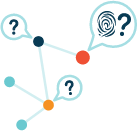
\includegraphics[width=0.2\textwidth]{Figures/svgviewer-png-output.png}
    \caption{Diagrama que explica la busqueda de un CID}
    \label{fg:looking_for_CID}
\end{figure}
Un usuario, puede anclar (pin) un fichero para guardar y proveer tu fichero para siempre. En cambio, los contenidos que no tengan ese pin serán descartados para liberar memoria. Esto significa que los usuarios solo guardan lo en lo que están interesados, mas un pequeño indice para saber que usuario tiene que.
Todos los ficheros van acompañados de un hash, haciendo que si alguien intenta cambiar el fichero o sus datos, resultara en un cambio en el hash. Esto implica que se le asignara un CID distinto. Esto significa que nuestros ficheros una vez subidos están seguros y serán resistentes ante la censura y la manipulación \ref{fg:keeping_IPFS_safe}.
\begin{figure}[h!]
    \centering
    
\includegraphics[width=0.2\textwidth]{Figures/svgviewer-png-output(2).png}
    \caption{Diagrama que explica la protección ante censura}
    \label{fg:keeping_IPFS_safe}
\end{figure}
\newpage
\thispagestyle{empty}